\begin{enumerate}[label=\arabic*.,ref=\theenumi]
%\begin{enumerate}[label=\thesection.\arabic*.,ref=\thesection.\theenumi]
\numberwithin{equation}{enumi}

\item

For the circuit in Fig. \ref{fig:ee18btech11051_fig1}, break the loop at node X and find the loop gain (working backward for simplicity to find $V_{X}$ in terms of $V_{O}$). For R = 10 k$\ohm$, find C and $R_{f}$ to obtain sinusoidal oscillations at 10 kHz.

\begin{figure}[!ht]
	\begin{center}
		\resizebox{\columnwidth}{!}{\begin{circuitikz}
\ctikzset{bipoles/length=1cm}

 
\draw (0, 0) node[op amp, scale = 0.5] (opamp) {};
\draw (opamp.-) --(-1,0.25)-- (-1,1) to[R=$R_{f}$,*-*] (1,1) -- (1,0);%[C=$C$,*-*] (0.25,-1) to [R=$R$,*-*] (-1,-1) -- (-1,-0.35) to (opamp.+);
\draw (opamp.+) --(-1,-0.25) to node[ground]{}  (-1, -0.6) ;
\draw (-1, 0.25) to [R=$R$,*-*] (-2.6, 0.25) to [C=$C$,*-*] (-2.6, -1.5) to node[ground]{} (-2.6,-2);
\draw (-2.6, 0.25) to [R=$R$,*-*] (-3.9, 0.25) to [C=$C$,*-*] (-3.9, -1.5) to node[ground]{} (-3.9,-2);
\draw (-3.9, 0.25) to [R=$R$,*-*] (-5.2, 0.25) to [C=$C$,*-*] (-5.2, -1.5) to node[ground]{} (-5.2,-2);
\draw (-5.2, 0.25) to [R=$R$,*-*] (-6.5, 0.25) -- (-6.5, 2) -- (1,2)-- (1,1);
\draw (opamp.out) -- (1.5,0) ;
\draw node at (1.8, 0){$V_{O}$};
\draw node at (-6.8, 0.25){X};
\end{circuitikz}
}
	\end{center}
\caption{}
\label{fig:ee18btech11051_fig1}
\end{figure}

\item
\solution
We first calculate the relation between $I_{4}$ and $V_{X}$ in fig \ref{fig:ee18btech11051_fig2} by using the relation between the currents and the fact that the inverting terminal of the Op-Amp is virtually grounded as follows:
\begin{figure}[!ht]
	\begin{center}
		\resizebox{\columnwidth}{!}{\begin{circuitikz}
\ctikzset{bipoles/length=1cm}


\draw (0, 0.25) to [C=$C$,*-*] (0, -1.5) to node[ground]{} (0,-2);
\draw (0, 0.25) to [R=$R$,*-*] (-2, 0.25) to [C=$C$,*-*] (-2, -1.5) to node[ground]{} (-2,-2);
\draw (-2, 0.25) to [R=$R$,*-*] (-4, 0.25) to [C=$C$,*-*] (-4, -1.5) to node[ground]{} (-4,-2);
\draw (-4, 0.25) to [R=$R$,*-*] (-6, 0.25);
\draw (0, 0.25) to [R=$R$,*-*] (2, 0.25);

\draw[-latex] (-6,0.25) to node[below] {$I_{1}$} (-5.6, 0.25);
\draw[-latex] (-4,0.25) to node[below] {$I_{2}$} (-3.6, 0.25);
\draw[-latex] (-2,0.25) to node[below] {$I_{3}$} (-1.6, 0.25);
\draw[-latex] (0,0.25) to node[below] {$I_{4}$} (0.4, 0.25);

\draw node at (-4, 0.5){$V_{1}$};
\draw node at (-2, 0.5){$V_{2}$};
\draw node at (0, 0.5){$V_{3}$};
\draw node at (2, 0.5){$V_{4}$};
\draw node at (-6, 0.5){$V_{X}$};
\end{circuitikz}
}
	\end{center}
\caption{}
\label{fig:ee18btech11051_fig2}
\end{figure}

Here, $V_{4}$ has zero voltage. Applying KVL between $V_{3}$ and $V_{4}$, we get
\begin{align}
    V_{3} = I_{4}R \label{eq:ee18btech11051_0}
\end{align}

Starting at node $V_{3}$ to node $V_{X}$, applying KCL and KVL sequentially, and substituting the previous two equations gives:\\
\begin{multline}
    I_{3} = I_{4} + V_{3}sC  \\  \implies I_{3} = I_{4}(1+sRC) 
\end{multline}
\begin{multline}
    V_{2} = V_{3} + I_{3}R  \\  \implies V_{2} = I_{4}R(2+sRC)
\end{multline}
\begin{multline}
    I_{2} = I_{3} + V_{2}sC\\
    \implies I_{2} = I_{4}(1+3sRC+(sRC)^{2}) 
\end{multline}
\begin{multline}
    V_{1} = V_{2}+ I_{2}R\\
    \implies V_{1} = I_{4}R(3+4sRC+(sRC)^{2})
\end{multline}
\begin{multline}
    I_{1} = I_{2} + V_{1}sC\\
    \implies I_{1} = I_{4}(1+6sRC+5(sRC)^2+(sRC)^3)
\end{multline}
\begin{multline}
    V_{X} = V_{1} + I_{1}R\\
    \implies V_{X} = I_{4}R(4+10sRC+6(sRC)^2+(sRC)^3)
    \label{eq:ee18btech11051_1}
\end{multline}

\begin{figure}[!ht]
	\begin{center}
		\resizebox{\columnwidth}{!}{\input{./figs/ee18btech11051/ee18btech11051_fig2.tex}}
	\end{center}
\caption{}
\label{fig:ee18btech11051_fig3}
\end{figure}
Also, As $V_{O} = -I_{4}R_{f}$, and using eq.\ref{eq:ee18btech11051_1}, we get
\begin{align}
    V_{O} = -V_{X}(\frac{R_{f}}{(4+10sRC+6(sRC)^2+(sRC)^3)R})
\end{align}

The oscillator doesn't have an input, but just a feedback loop with an infinite gain to create oscillations. So, comparing the circuit structure from fig.\ref{fig:ee18btech11051_fig3}, we get
\begin{align}
    G(s)H(s) = \frac{V_{O}}{V_{X}} = \frac{R_{f}}{(4+10sRC+6(sRC)^2+(sRC)^3)R}\label{eq:ee18btech11051_2}
\end{align}

where, H(s) = 1. To make the system oscillate at a frequency $\omega_{O}$, the phase shift of the loop should be zero, and poles on the imaginary axis
\begin{align}
    |GH|=1\\ \angle GH = 0^{\degree} \\
    \implies (\omega RC)^{2} = 10 \label{eq:ee18btech11051_3}
\end{align}

After calculating the values of $R_{f}$ and C from eq.\ref{eq:ee18btech11051_2} and eq.\ref{eq:ee18btech11051_3} respectively, the values are:
\begin{table}[!ht]
    \centering
    \input{./tables/ee18btech11051/ee18btech11051_table1.tex}
    \caption{Final Values}
    \label{table:ee18btech11051_table_1}
\end{table}

\item
Verification:\\
The value of $R_{f}$ is kept slightly above the calculated value for the system to start the oscillations. The impluse response of the resulting transfer function is plotted in fig.\ref{fig:ee18btech11051_plot1} using the plot in 
\begin{lstlisting}
codes/ee18btech11051/ee18btech11051_1.py
\end{lstlisting}

\begin{figure}[!ht]
\centering
\includegraphics[width=\columnwidth]{./figs/ee18btech11051/ee18btech11051_plot1.eps}
\caption{Impulse Response in python}
\label{fig:ee18btech11051_plot1}
\end{figure}

The circuit simulated in Spice can be found in
\begin{lstlisting}
codes/ee18btech11051/spice/ee18btech11051_spice.asc
\end{lstlisting}
and the python code used for plotting the data is
\begin{lstlisting}
codes/ee18btech11051/ee18btech11051_2.py
\end{lstlisting}

\begin{figure}[!ht]
\centering
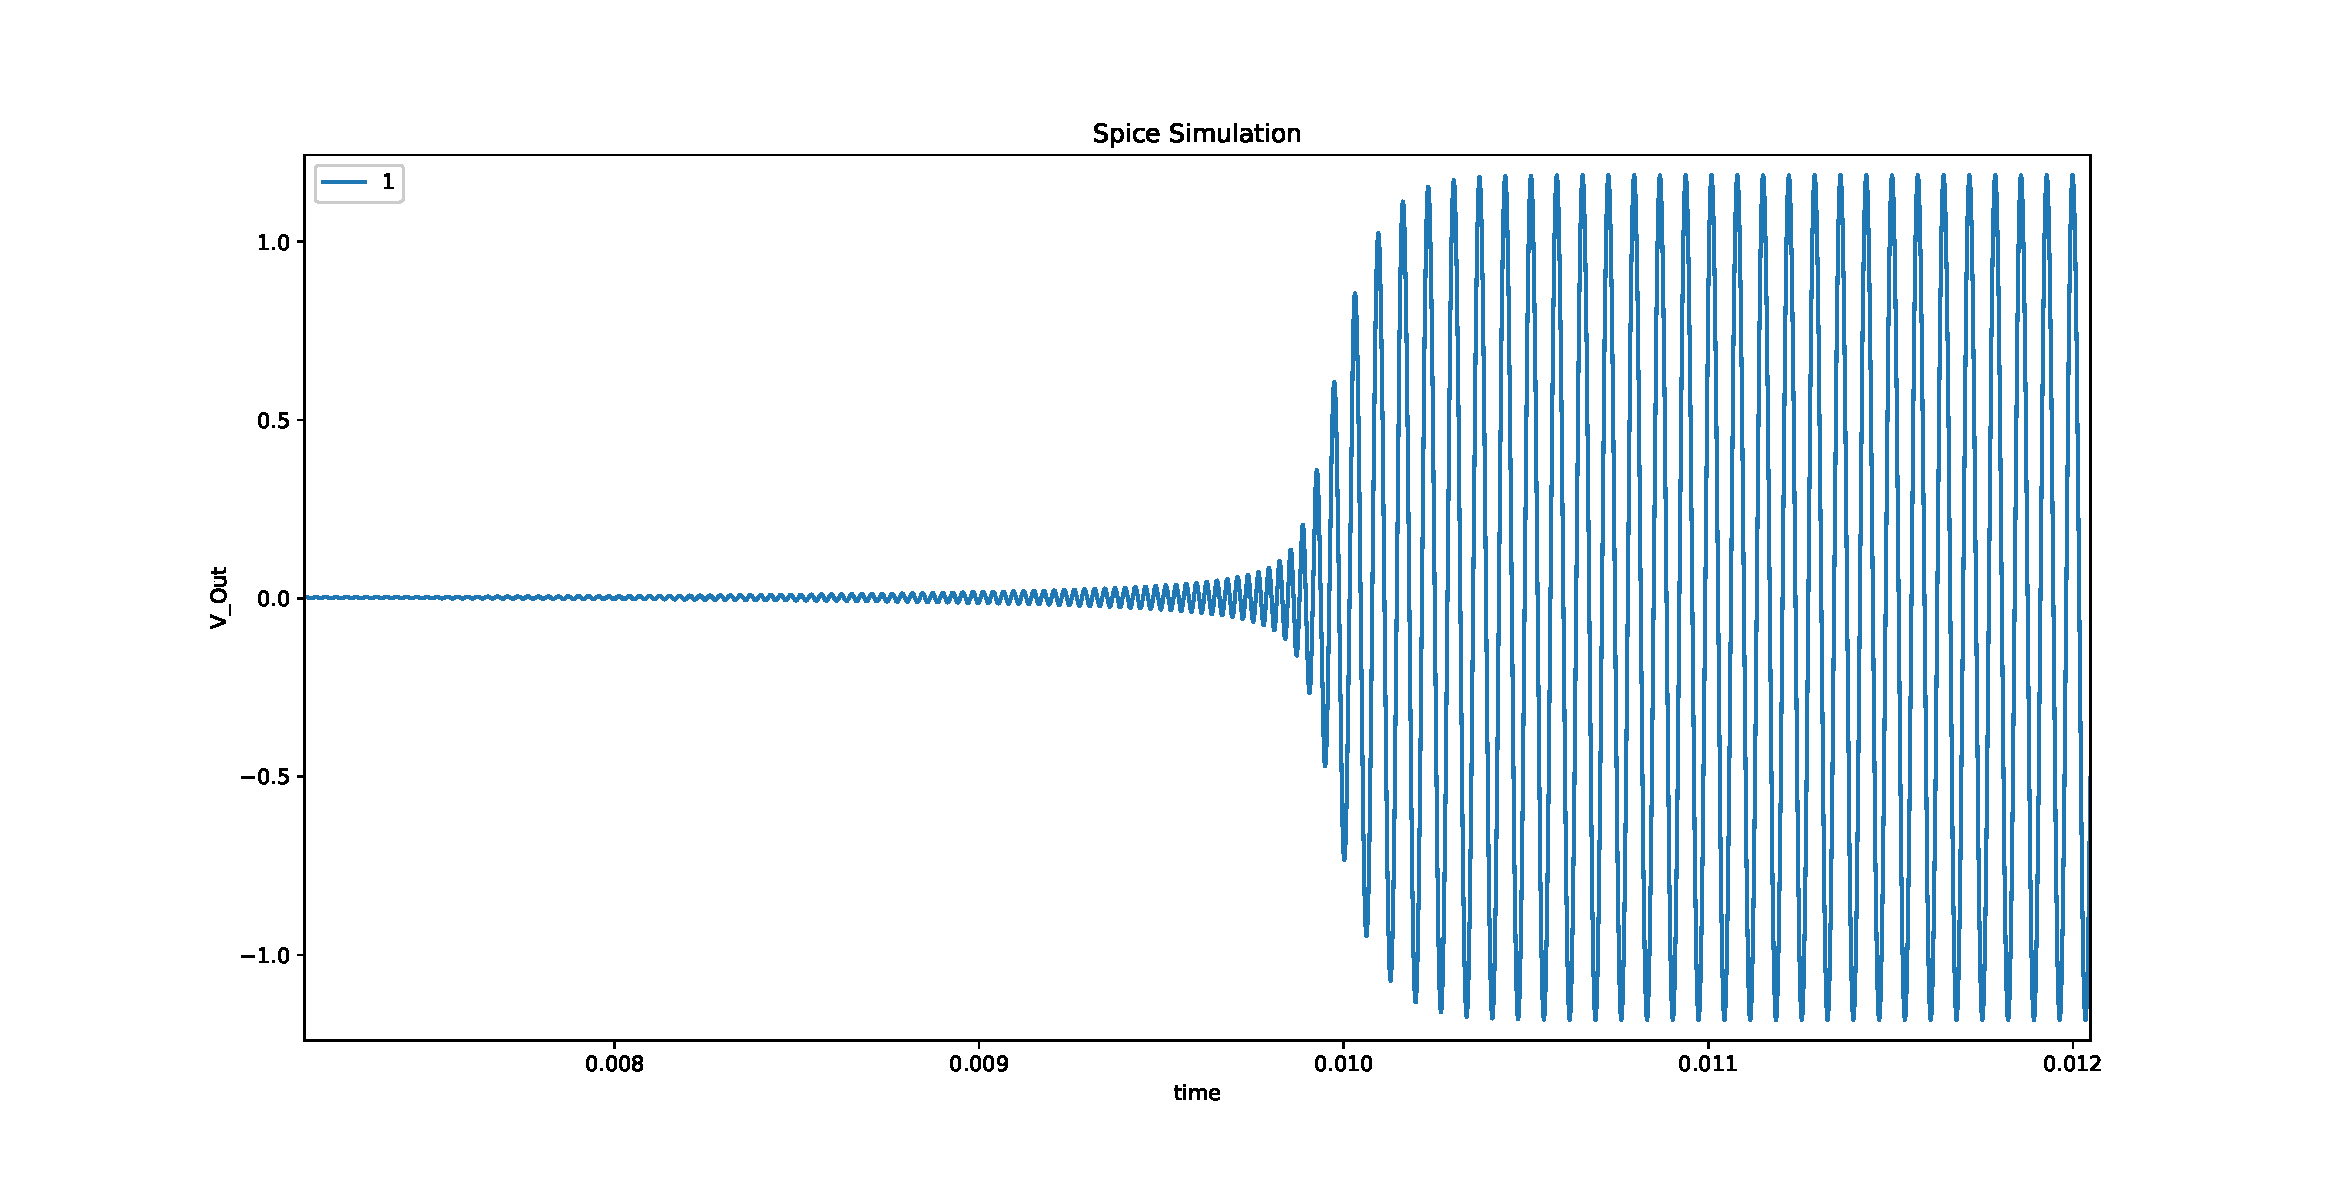
\includegraphics[width=\columnwidth]{./figs/ee18btech11051/ee18btech11051_plot2.eps}
\caption{Spice Simulation}
\label{fig:ee18btech11051_plot2}
\end{figure}
To verify the frequency of the oscillator, we measure the time lapse between two peaks as shown in fig.\ref{fig:ee18btech11051_plot3}
\begin{figure}[!ht]
\centering
\includegraphics[width=\columnwidth]{./figs/ee18btech11051/ee18btech11051_plot3.eps}
\caption{}
\label{fig:ee18btech11051_plot3}
\end{figure}
The points are (0.0108666, 1.1862) and (0.0109585, 1.1906). So, the time interval between peaks is 0.0109585 - 0.0108666 = 0.0000919.
So, achieved $f_{O} = \frac{1}{0.0000919} = 10.8kHz$.
Hence, the design is achieved.

\end{enumerate}
